The hardware for the Data Acquisition and Stimulation System requires several supply voltages to power the digital integrated circuits (ICs) in addition to dual analog power supplies for amplification circuitry.  Consequently, there are several options for providing power to the Real Time System Controller Board and Electrophysiology Interface board.  Figure~\ref{fig:Power} summarizes the power needs of the ICs and circuit blocks along with the power input connectors and voltage regulators.

\begin{figure}[H]
	\begin{singlespace}
	\centering 
		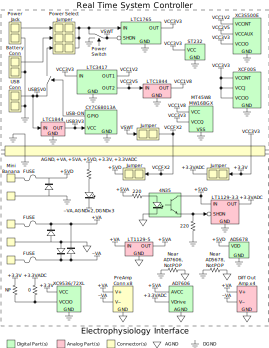
\includegraphics{./figures/Power} 
	\caption{Power connectors and IC power connections on the Real Time System Controller Board~\cite{DigilentNexys2rm,DigilentNexys2sch} and the Electrophysiology Interface board\label{fig:Power}}
	\end{singlespace}
\end{figure}

\subsubsection{Real Time System Controller Power}\label{sec:rtscpower}

The RTSC has selectable input power options configured by placing a jumper connecting the desired power connector to a LTC1765 switching voltage regulator.  The power jack and battery connector both connect directly to the regulator, but the CY7C68013A Cypress microcontroller, which requires a $+3.3\unit{V}$ supply and acts as the USB PHY, draws power exclusively from the USB interface, so a LTC1844 linear regulator is included to regulate the $+5.0\unit{V}$ USB input voltage to the required value.  When a USB cable is connected to the RTSC and a PC, the Cypress microcontroller informs the PC that more than $100\unit{mA}$ of current will be drawn over the USB interface; then, the USB$-$ON signal switches a NMOS transistor, connecting USB power, which can supply up to $500\unit{mA}$ of current, to the power selection jumper~\cite{DigilentNexys2rm,DigilentNexys2sch}.  The power consumption of the RTSC will vary based on the configuration of the Xilinx\textsuperscript{\textregistered} XC3S500E FPGA, clock speeds of the digital logic, and the power drawn from the Electrophysiology Interface board~\cite{DigilentNexys2rm}.

The power switch on the RTSC board connects the active low shutdown signal ($\overline{\mathrm{SHDN}}$) of the LTC1765 regulator to either the power selection jumper (to enable the regulator output) or to ground (to disable the regulator output)~\cite{LT1765ds}.  Setting the power switch to the off position does not disconnect USB power from the Cypress microcontroller but does disconnect the main power jumper from VCCFX2 if the jumper is in place to connect the VSWT to VCCFX2~\cite{DigilentNexys2sch}.

Most of the circuits on the RTSC board are powered by the VCC3V3 supply, which is why a LTC1765 high-efficiency switching regulator is used for the supply.  The ST232 RS232 level shifting IC and the Xilinx\textsuperscript{\textregistered} Platform Flash XCF00S configuration flash memory require only 3.3V~\cite{ST232ds,XilinxPlatformFlashDS}.  The Xilinx\textsuperscript{\textregistered} Spartan 3E XC3S500E FPGA requires a significant amount of current at $+1.2\mathrm{V}$ for its internal core, VCCINT, and requires $+2.5\unit{V}$ for its auxiliary supply voltage, VCCAUX, so a LTC3417 high-efficiency dual-output switching regulator provides the needed supply voltages~\cite{DigilentNexys2rm,Spartan3eDS}.  Also, the MT45W8MW16BGX 128Mb DRAM module alone requires a $1.8\unit{V}$ core voltage, with a maximum current of $25\unit{mA}$ at $66\unit{MHz}$ and $45\unit{mA}$ at $133\unit{MHz}$, along with an IO voltage supply equal to the FPGA IO voltage~\cite{MicronDRAMds}.  Thus, a LTC1844 linear regulator is provided for the specialized VCC1V8 voltage supply, and since linear regulator efficiency is directly proportional to the magnitude of the voltage drop across the regulator, it is powered by the voltage supply that will require the least voltage drop, VCC2V5~\cite{DigilentNexys2sch}.

\subsubsection{Electrophysiology Interface Power}

To isolate analog devices from the noise generated by digital devices, it is preferable to have separate power supplies and ground for the digital and analog devices on the Electrophysiology Interface board.  In addition, the Preamp boards connected also draw power from the analog voltage supplies on the Electrophysiology Interface board.

The integrated circuits requiring a digital voltage supply are the Analog Devices AD5678 DAC, the Xilinx\textsuperscript{\textregistered} XC9536/72XL CPLD, and the logic supply, VDrive, of the AD7606 ADC.  The nine LT1124 dual op-amp ICs of the differential output amplifier blocks require dual analog voltage supplies, and each Preamp requires dual analog voltage supplies for its LT1167 instrumentation amplifier, LT1124 dual op-amp, LT1125 quad op-amp, and ADG202 analog switch ICs.  Complicating the analog voltage supply requirements is the Analog Devices AD7606 ADC, which requires a $+5.0\mathrm{V} \pm 0.25\unit{V}$ analog voltage supply, AVCC~\cite{AD7606ds}.

Five 2mm banana (also known as mini-banana) connectors are provided on the Electrophysiology Interface board to connect analog voltage ($\pm \mathrm{VA}$) and ground (AGND) and digital voltage (+5VD) and ground (DGND).  The magnitude of +VA should be a close as possible to the magnitude of $-\mathrm{VA}$.  Table~\ref{tab:powerinput} shows the acceptable voltage range of the power supply inputs.  The minimum and maximum values of +5VD are determined by the AD5678 requirements, but it should be noted that the maximum DAC output voltage will be equal to the supply voltage~\cite{AD5678ds}.  The minimum value for the $\pm \mathrm{VA}$ supply is determined by the dropout voltage of the LT1129-5 regulator ($0.45\unit{V}$ at $100\unit{mA}$ load current~\cite{LT1129ds}), and the maximum value for the $\pm \mathrm{VA}$ supply is limited by the requirements of the LT1167 instrumentation amplifier and ADG202 analog switches on the Preamp boards~\cite{LT1167ds,ADG202Ads}.

\renewcommand{\arraystretch}{1.3}
\begin{table}[h]
\centering
\begin{tabular}{|l|l|l|l|}
\hline
Supply & TYP (V) & MIN (V) & MAX (V)\\
\hline
+5VD & 5.0 & 4.5 & 5.5\\
\hline
$|\pm \mathrm{VA}|$ & 9.0 & 5.5 & 15.0\\
\hline
\end{tabular}
\caption{Electrophysiology Interface power supply voltages\label{tab:powerinput} }

\end{table}
\renewcommand{\arraystretch}{1.0}

Fuses and protection diodes will protect the circuits on the Electrophysiology Interface board if the supply leads are reversed.  If the supply leads are reversed, one or more of the protection diodes will be forward biased, allowing a large amount of current to flow between the reversed supply leads causing a fuse to blow and the dangerous voltage to be disconnected from the rest of the board.  The fuses on the Electrophysiology Interface board are surface mount fuses in 0805 packages that have the advantage of taking up very little board space but have the disadvantage of having a high series resistance of $0.7\unit{\Omega}$ (measured).  When one of the fuses blows, it is not visually distinguishable from a non-blown fuse.  To ensure a low resistance connection, the ground connection does not go through a fuse, which will present a problem if a power lead is connected to a ground connector that creates a large voltage difference between the analog and digital grounds.

The $3.3\unit{V}$ supply from the RTSC board is used to power the core of the CPLD and may be used to power the IO buffers of the CPLD and ADC by connecting the jumper from $+3.3\unit{V}$ to +3.3VADC, in which case the LT1129-3.3 should not be populated.  Alternatively, the IO buffer of both the ADC and CPLD or the ADC alone may be powered by a LT1129-3.3 linear regulator that converts the +5VD voltage to $3.3\unit{V}$.  To ensure that the IO buffers of the ADC are powered only when the ADC's AVCC is powered and to preserve analog and digital isolation, a 4N35 opto-isolator, with its input driven by the $+5\mathrm{VA}$ supply, controls the operation of the linear regulator.  Since other signals from the CPLD and DAC violate analog and digital isolation, as discussed in section~\ref{sec:ground}, the opto-isolator is excessive, but it illustrates the concept of analog and digital isolation.

Both the AD5678 DAC and the AD7606 ADC recommend analog and digital ground and power isolation, but when analog and digital grounds are to be connected at some point, the connection should be as close as possible to the AD5678 as recommended by~\cite{AD5678ds}, and the connection should be as close as possible to the AD7606 as recommended by~\cite{AD7606ds}.  To accommodate this conflicting information, pads for $0\unit{\Omega}$ resistors are provided near the DAC and ADC for testing analog and digital ground connections.  Although, with all of the signals that connect analog and digital powered devices, as discussed in section~\ref{sec:ground}, a single $0\unit{\Omega}$ resistor may not be sufficient for routing signal return currents.

The +5VD supply may be configured to be powered by the main input bus of the RTSC board by connecting the jumper on the RTSC the connects VSWT to VCCFX2 and the jumper on the Electrophysiology Interface board that connects VCCFX2 to +5VD.  The reverse should not be practiced: using +5VD to power the RTSC could result in the +5VD power supply being shorted to ground by the power switch that connects VSWT to the main input bus or to ground.  If the USB interface is used to power the RTSC and the Electrophysiology Interface boards, care must be taken to ensure that no more than $500\unit{mA}$ is drawn from the USB interface.  A typical configuration of the FPGA may cause the RTSC, itself, to draw $300\unit{mA}$ of power from the USB interface~\cite{DigilentNexys2rm}.  The AD5678 draws only $2.6\unit{mA}$ of quiescent current with its internal voltage reference on, but the AD5678 output amplifiers draw varying amounts of current based on input resistance of the Differential Output Amplifier blocks~\cite{AD5678ds}.  The CPLD's power consumption varies depending on its configuration and clock speed.  With a configuration consisting entirely of 16-bit counters, a XC9536XL can draw between $15\unit{mA}$ and $65\unit{mA}$ of current from the $+3.3\unit{V}$ power supply, and a XC9572XL can draw between $25\unit{mA}$ and $125\unit{mA}$~\cite{XC9536XLds,XC9572XLds}.  The resulting current drawn from the USB interface depends on the power efficiency of the LTC1765, which varies from 75\% to 87\% depending on output current~\cite{LT1765ds}.

LEDs are provided to give a visual indication for each power supply to which they are connected.  The LEDs are driven by the power supply rail through a resistor to limit the current through each LED.  The magnitude of the resistance is determined based on the desired current in the LED and the forward voltage of the LED.  Red surface mount LEDs from Kingbright are used that have a rated forward current of $\mathrm{I}_\mathrm{F}=20\unit{mA}$ with a forward voltage of $\unit{V}_{\mathrm{FTyp}}=2.0\unit{V}$~\cite{RedKingbrightLEDds}.  A forward current of $\mathrm{I}_\mathrm{F}=5\unit{mA}$ is bright enough for an indicator.  Using the constant-voltage-drop model of the diode, a resistance values is calculated, using

\begin{equation}
\label{equ:ledres}
R = \frac{(\mathrm{V}_{\mathrm{supply}} - \mathrm{V}_{\mathrm{F}})}{\mathrm{I}_\mathrm{F}},
\end{equation}
to produce the desired forward current based on the power supply voltage, $\mathrm{V}_{\mathrm{supply}}$, and the typical forward voltage of the diode, $\mathrm{V}_\mathrm{F}$.  For example, the power supplies with a nominal voltage of $\unit{V}_{\mathrm{supply}}=+5.0\unit{V}$, using $\mathrm{I}_\mathrm{F}=5\unit{mA}$ and $\mathrm{V}_\mathrm{F}=\mathrm{V}_{\mathrm{FTyp}}=2.0\unit{V}$ yields a resistance of $R=600\unit{\Omega}$.  A standard value resistor that is $560\unit{\Omega}$, which is close to $600\unit{\Omega}$, is populated on the Electrophysiology Interface board for the LEDs that indicate the +5VD and $+5\mathrm{VA}$ supplies are on.  For the $\pm \mathrm{VA}$ supplies, a resistance value is populated that will yield forward currents below the maximum specified for the part for the range of input voltages specified in Table~\ref{tab:powerinput}.


\subsubsection{Linear Regulator Thermal Consideration}

To produce the $+5.0\unit{V}$ analog voltage required by the AD7606, an LT1129-5 linear regulator is provided.  The LT1129-5 produces a $+5.0V \pm 150mV$ voltage that meets the requirements of the AD7606~\cite{LT1129ds}.  Linear regulators offer excellent noise characteristics and circuit simplicity compared to switching regulators; the trade off is low efficiency, which can result in a significant amount of heat in the regulator that must be considered.  The maximum allowed junction temperature of the LT1129 series is $125 ^\circ \unit{C}$~\cite{LT1129ds}.  To estimate the junction temperature, the junction-to-ambient thermal resistance of the IC package, $\mathrm{R}_{\mathrm{TH}}$ given in $^\circ \unit{C} / \unit{W}$, is multiplied by the power dissipation of the part~\cite{LT1129ds}.  Two equations describe the amount of power (heat) dissipated in a voltage regulator.  The power dissipated due to the current drawn by the circuit connected to the regulator output is
\begin{equation}
\label{equ:Pdrop}
\mathrm{P}_{\mathrm{drop}} = \mathrm{I}_{\mathrm{OUT}} (\mathrm{V}_{\mathrm{IN}} - \mathrm{V}_{\mathrm{OUT}}),
\end{equation}
which, according to Kirchoff's Current Law, has to come from the input, and 
\begin{equation}
\label{equ:Pgnd}
\mathrm{P}_{\mathrm{gnd}} = \mathrm{I}_{\mathrm{GND}} \times \mathrm{V}_{\mathrm{IN}}
\end{equation}
is the power dissipated by the current flowing from the input to ground where $\mathrm{I}_{\mathrm{GND}}$ is estimated based on performance curves in~\cite{LT1129ds}.


Since the AD7606 is the most significant current draw on the output of the LT1129-5, the supply current given in the AD7606 data sheet is used to estimate the current draw on the LT1129-5.  The AD7606 data sheet specifies that, when the device is operational, the maximum supply current is 27mA~\cite{AD7606ds}.  Thus, the expected maximum power dissipated in the LT1129 is $\mathrm{P}_{\mathrm{drop}} + \mathrm{P}_{\mathrm{gnd}} = 276\unit{mW}$ based on one eight channel AD7606 drawing $27\unit{mA}$ for $\mathrm{I}_{\mathrm{OUT}}$, $\mathrm{V}_{\mathrm{IN}}$ provided by $+\mathrm{VA}$ at the maximum $15\unit{V}$, and $\mathrm{I}_{\mathrm{GND}}$ estimated to be $0.6\unit{mA}$ based on performance curves in~\cite{LT1129ds}.

The junction-to-ambient thermal resistance depends on the IC package and the area of copper in the PCB that will spread the heat away from the IC~\cite{LT1129ds}.  Taking the worst thermal characteristic package, 8-pin SOIC with $100\unit{mm}^2$ of copper on the top side of the board and $2500\unit{mm}^2$ on the bottom side of the board with $\mathrm{R}_{\mathrm{TH}}=69^\circ \unit{C} / \unit{W}$~\cite{LT1129ds}, yields a temperature rise of $276\unit{mW} \times 69^\circ \unit{C} / \unit{W} = 19.0^\circ \unit{C}$, which means that, in the worst case scenario, the junction temperature of the LT1129 will only be $19.0^\circ \unit{C}$ warmer than the ambient temperature.  Since the ambient temperature would have to be above $106^\circ \unit{C}$ to yield a junction temperature that could damage the part, it is safe to choose the 8-pin SOIC package for the $+5\mathrm{VA}$ regulator.
